%%%%%%%%%%%%%%%%%%%%%%%%%%%%%%%%%%%%%%%%%%%%%%%%%%%%%%%%%%%%%%%%%%%%%%%%%%%%%%%%%%%%%%%%%%%%%%%%%%%%%%%%%%%%%%%%%%%%%%%%%%%%%%%%%%%%%%%
%%Latexvorlage by Pascal Enderli, Zürich
%%%%%%%%%%%%%%%%%%%%%%%%%%%%%%%%%%%%%%%%%%%%%%%%%%%%%%%%%%%%%%%%%%%%%%%%%%%%%%%%%%%%%%%%%%%%%%%%%%%%%%%%%%%%%%%%%%%%%%%%%%%%%%%%%%%%%%%
%% Diese Vorlage enthät alle nötigen tools um ein grosses Projekt (Bachelorarbeit, Masterarbeit) zu verfassen.
%% Unter anderem ist enthalten:
%% -struktur einer wissenschaftlichen arbeit
%% -abbildungs-,tabellen-,literatur-,akronym- und symbolverzeichnis
%% -Makefile für offlinekompilierung (Linuxuser) ausführen mit ./make.sh im obersten ordner
%% -einige befehle und hinweise für die verwendung von referenzen aller art im file:
%% ./mainmatter/introduction.tex und ./backmatter/literature.bib
%%%%%%%%%%%%%%%%%%%%%%%%%%%%%%%%%%%%%%%%%%%%%%%%%%%%%%%%%%%%%%%%%%%%%%%%%%%%%%%%%%%%%%%%%%%%%%%%%%%%%%%%%%%%%%%%%%%%%%%%%%%%%%%%%%%%%%%
%% Bemerkungen:
%% Das Skript darf natürlich nach euren wünschen angepasst und wiederveröffentlicht werden
%% Bei der Erstellung des Literaturverzeichnisses habe ich biber verwendet (weil utf-8 kompatibel),
%% welches vor dem kompilieren nachinstalliert werden muss falls noch nicht vorhanden (unter linux: sudo apt-get install biber )
%% alternativ kann man das projekt auf sharelatex.com hochladen und bearbeiten
%% (bitte sicher stellen dass das file ./frontmatter/glossaries.glo korrekt in sharelatex importiert wurde)
%% Dieses Skript verwendet KOMA-Skript 
%%%%%%%%%%%%%%%%%%%%%%%%%%%%%%%%%%%%%%%%%%%%%%%%%%%%%%%%%%%%%%%%%%%%%%%%%%%%%%%%%%%%%%%%%%%%%%%%%%%%%%%%%%%%%%%%%%%%%%%%%%%%%%%%%%%%%%%

\documentclass[
parskip=full,               %ganze leere linie vor neuen absatz <false(einzug),half halbe linie abstand>
headings=small,             %kleinere schrift bei den kopfzeilen
headsepline=0.3pt,          %separierungslinie für kopfzeile <dicke:länge>
footsepline=false,          %separierungslinie für fusszeile <dicke:länge>
plainheadsepline=true,      %separierungslinie für kopfzeile auch bei seite mit neuem kapitel
plainfootsepline=false,     %separierungslinie für fusszeile auch bei seite mit neuem kapitel
11pt,                       %schriftgrösse <10pt, 11pt, 12pt>
oneside,                    %modus einseitige seiten <twoside>
a4paper                     %a4 format
]{scrbook}                  %komaskript klasse scrbook


\usepackage{header}

%%%%%%%%%%%%%%%%%%%%%%%%%%%%%%%%%%%%%%%%%%%%%%%%%%%%%%%%%%%%%%%%%%%%%%%%%%%%%%%%%%%%%%%%%%%%%%%%
%auswählen welche files kompiliert werden sollen (Auskommentieren)

\includeonly{
./frontmatter/Titlepage,            
./frontmatter/Declaration,
./frontmatter/Abstract,           
./mainmatter/Demo,  
./mainmatter/Introduction,
./mainmatter/Theory,
./mainmatter/Methods,
./mainmatter/Results,
./mainmatter/Discussion,
./mainmatter/Conclusion,
./backmatter/Appendix   
}
%%%%%%%%%%%%%%%%%%%%%%%%%%%%%%%%%%%%%%%%%%%%%%%%%%%%%%%%%%%%%%%%%%%%%%%%%%%%%%%%%%%%%%%%%%%%%%%%
%%%%%%%%%%%%%%%%%%%%%%%%%%%%%%%%%%%%%%%%%%%%%%%%%%%%%%%%%%%%%%%%%%%%%%%%%%%%%%%%%%%%%%%%%%%%%%%%
%erzeugen des Dokumentes

%Frontmatter
\begin{document}
\sloppy
% Titelseite gefolgt von einer leeren seite 


%Hinweise zum Deckblatt:
% Aussagekräftige Titel und Untertitel
%Projektgruppe (Namen), Nennung der Verantwortlichen
%Institution (gegebenenfalls mit Logo) 
%Datum, Semesterbezeichnung
%Grafik (optional) – wenn, dann aussagekräftig!

% Kann auch als includepdf mit einem andersweitig erstelten Titelblatt realisiert werden




\begin{titlepage}
\begin{center}
    \vspace*{1cm}
    {\huge \bfseries Titel der Arbeit \\ }
    \vspace{2cm}
    {\large 
	Name\\

	~\\
	Mechanical Engineering Bachelor\\
	\vspace{3.5cm}
	Fokusprojekt HS 2015; FS 2016\\
	~\\
	Name des Institutes\\
	ETH Zürich\\
    }

\vspace{\stretch{1}}



{\large
	Supervisors: \\[\baselineskip]
	Name\\
	Name\\[1cm]


	
	Professor:\\[\baselineskip]
	Prof. Dr. Name
}
\end{center}

\vspace*{2cm} % a bit of space at the bottom of the page

\end{titlepage}


%\clearpage\null


% Einfügen einer leeren Seite nach dem Titelblatt
\begin{titlepage}
\thispagestyle{empty}
\newpage
\mbox{}
\end{titlepage}
\chapter*{Abstract}

\section*{Initial situation}
\section*{Results}



\cleardoublepage                                        %alle gleitobj. ausgeben und wechsel auf rechte seite
\tableofcontents
\cleardoublepage
\printglossary[title=Nomenclature,toctitle=Nomenclature,style={mystyle}]
\cleardoublepage
\printglossary[type=\acronymtype,title=Acronyms,toctitle=Acronyms]

%ABBILDUNGSVERZEICHNIS
\cleardoublepage                                       
\phantomsection                                        %referenziert hyperrefs an diese stelle
\addcontentsline{toc}{chapter}{List of Figures}        %manueller Eintrac im table of content (TOC)
\listoffigures

%TABELLENVERZEICHNIS
\cleardoublepage
\phantomsection
\addcontentsline{toc}{chapter}{List of Tables}
\listoftables

%Mainmatter                                             \chapter \section \subsection \subsubsection 
\mainmatter	                                            %arabische Seitenzahlen
\chapter{Demo}\label{chp:demo}
\section{aaa}\label{sec:aaa}
\subsection{bbb}
\subsubsection{ccc}


Demonstration der Quellenangaben, Akronym- und Symbol- Referenzierung

Die Farben der Verlinkungen können im File header.sty geändert werden.

Eine einfache Referenz ins Literaturverzeichnis\cite{einstein}\\

\textcquote{einstein}{Dies ist ein Zitat}\\
\blockcquote{einstein}{Dieses Zitat ist im Displaymode}

Nachher kommt die Fussnote\footnote{footnotes working fine}\\

Hier verwende ich das Symbol \gls{pi},\gls{rho} und \gls{p} das geht auch im
Mathematik Modus \\

$$\gls{rho}$$

Und hier eine Abkürzung \gls{eth}\\
Bei der zweiten Verwendung steht nur noch die Abkürzung ohne Erklärung
\gls{eth}\\[5mm]

Einheiten werdern so verwendet: \SI{2}{m}

Das ist ein Beispieltext, der automatisch umgebrochen werden sollte. Ich hoffe
das hat keinen Einfluss auf das finale Dokument. Denn da möchte ich eher ein
Softwrap als ein hart. Dieser Text ist jetzt ziemlich sicher lang genug, um
diesen Effekt zu zeigen. Dieser Effekt tritt vor allem dann auf, wenn der Text
sehr lange wird. Andri geht heute noch fischen und steht dabei nackt auf dem
Boote.

Eine Aufzählung:
\begin{itemize}
    \item Bla
\end{itemize}


\begin{figure}[H]
    \centering
    
\includegraphics[width=0.5\textwidth]{./mainmatter/pictures/Demo/kolibri-logo}
    \caption{The logo of the Kolibri}
    \label{Kolibri}
\end{figure}


\begin{table}[H]
\centering
\begin{tabular}{|c|c|c|}
	\hline & Messbereich & Auflösung\\ 
	\hline Fx & 80N   & 1/50N\\ 
	\hline Fy & 80N   & 1/50N\\ 
	\hline Fz & 240N  & 1/25N\\ 
	\hline Mx & 4Nm   & 1/2000Nm\\ 
	\hline My & 4Nm   & 1/2000Nm\\ 
	\hline Mz & 4Nm   & 1/2000Nm\\
	\hline 
\end{tabular} 
\caption{das ist eine Tabelle}
\label{tbl:Tabelle}
\end{table}


Ich kann auch auf das Bild verweisen (\autoref{Kolibri})\\
oder auf den Anhang: \autoref{app:codeofconduct} \\
oder auf das Kapitel: \autoref{chp:demo}\\
oder auf die section: \autoref{sec:aaa}\\
Wenn ich nur die Nummer ohen Keyword will, dann nehme ich \ref{chp:demo}

\chapter{Introduction}
\chapter{Theory}
\chapter{Methods}

\begin{lstlisting}[language=js]
const f = (x,y) => {
		console.log(x+y);
}
\end{lstlisting}

\chapter{Results}
\chapter{Discussion}
\chapter{Conclusion}


%Backmatter
\cleardoublepage
\printbibliography[                                     %Literaturverzeichnis
heading=bibintoc,                                       %Literaturverzeichnis in Inhaltsverzeichnis auflisten
title={Bibliography}]                                   %Titel des Literaturverzeichnisses
\renewcommand{\chaptermark}[1]{         		        %Kopfzeile wird von Kapitel zu Anhang umbenannt
\markboth{Appendix\ \thechapter: #1}{}}                 
\begin{appendices}                                      %umfangreichere variante als \appendix
\clearpage
%Die Erste Seite mus getrennt eingebunden werden. mit dem pagecommand (titel und label für referenzen)
%jede weitere Seite dann ohne pagecommand.
% 2- steht für seite zwei und folgende
% 2-5 steht für seite 2-5

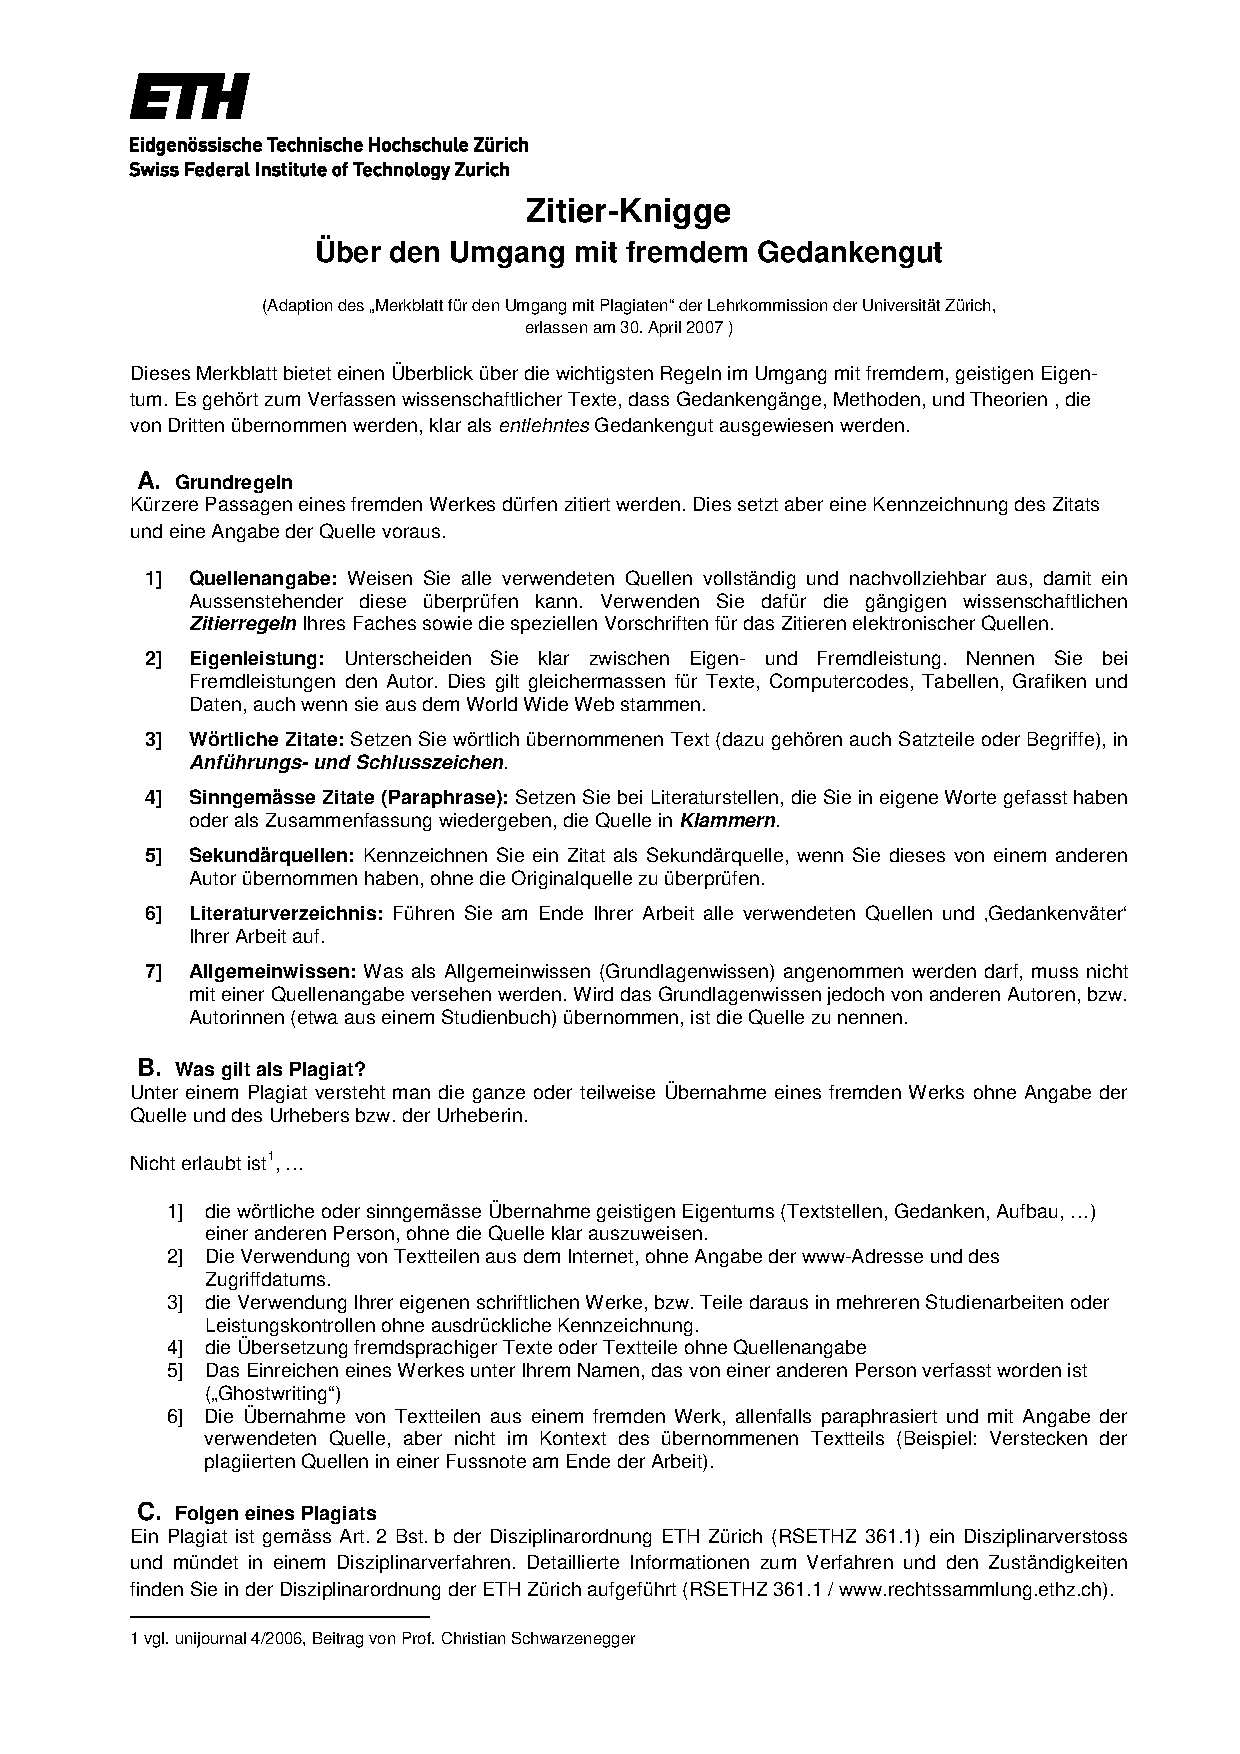
\includepdf[scale=0.75,angle=00,offset=0mm -18mm,pages={1},frame=true,pagecommand={\chapter{Code of Conduct}\label{app:codeofconduct}}]{./backmatter/pictures/plagiat}
\includepdf[scale=0.75,pages={2-},frame=true,pagecommand={}]{./backmatter/pictures/plagiat}

\end{appendices}


\end{document}